\section*{Aufgabe 4.1a)}
\begin{lstlisting}[caption=Output des Beispielaufrufs,label=lst:fouriertestoutput,language=]
Vektor eins: 
v1 =

   1
   2
   3
   4
\end{lstlisting}



\section*{Aufgabe 5.1}
Im Folgenden wurde mittels der Fourier-Analyse eine Möglichkeit der Bildkomprimierung
getestet. Das in Matlab als $(m\times n)$-Matrix importierte Bild ohne Veränderungen ist
in \fref{orig} abgebildet. Die Matrix enthält die Graustufenwerte als Fließkommazahlen
(\texttt{double}).

\begin{figure}[htb]
\centering
  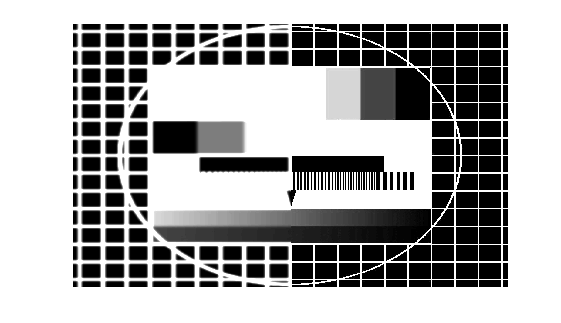
\includegraphics[width=0.7\textwidth,keepaspectratio]{../tmp/original}
  \caption{Orginales Bild ohne Komprimierung}
  \label{fig:orig}
\end{figure}

\section*{Aufgabe 5.1a)}

Zunächst wurde eine Funktion \lref{cut_rect} geschrieben, die den Rand des Graustufen-Bildes
schwärzt, die Pixel also auf 0 setzt. Die Breite wird hierbei in Abhängigkeit
des Kompressionsparameters $ρ \in [0,1]$ so eingestellt, dass $hb\cdot ρ^2$
nicht-triviale Pixel verbleiben, wobei $h$ die Höhe und $b$ die Breite des
Bildes in Pixeln ist.

\lstinputlisting[firstline=1,lastline=10,firstnumber=1,label=lst:cut_rect,caption={cut\_rect.m}]{../code/cut_rect.m}

Wird die Funktion aus \lref{cut_rect} unter Verwendung von $ρ^2 = 0.4$ auf das
Bild in \fref{orig} angewendet, so erhält man die in \fref{1a} gezeigte Abbildung.

\begin{figure}[htb]
\centering
  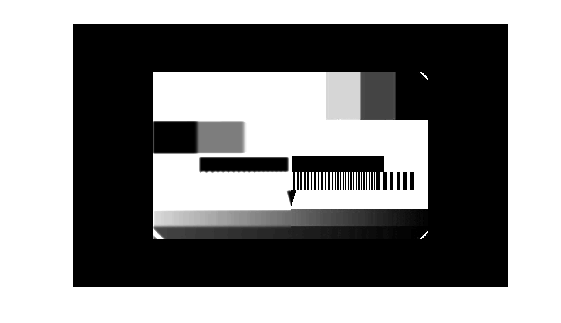
\includegraphics[width=0.7\textwidth,keepaspectratio]{../tmp/eins_a}
  \caption{Bild mit Rand bei $ρ^2 = 0.4$}
  \label{fig:1a}
\end{figure}

\section*{Aufgabe 5.1b)}
\section*{Aufgabe 5.1c)}

Zur Komprimierung des Bildes aus \fref{orig} wird eine 2D-Fourier-Transformation
in den $k$-Raum durchgeführt. Im Anschluss wird das Bild symmetrisiert, die Bildinformation
auf $hb\cdot ρ^2$ durch das Abschneiden des Randes reduziert, die Symmetrisierung wieder
rückgängig gemacht und zuletzt wird das Bild wieder durch die inverse Fourier-Trafo in den
$x$-Raum überführt.

Das Ergebnis für $ρ=0.5$ ist in \fref{1c5} und für $ρ=0.1$ ist in \fref{1c1} dargestellt.

\begin{figure}[htb]
\centering
  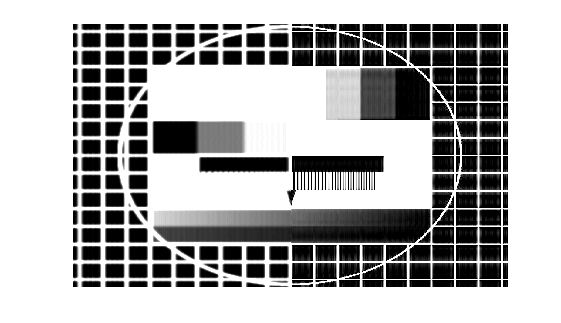
\includegraphics[width=0.7\textwidth,keepaspectratio]{../tmp/eins_c_0_5}
  \caption{komprimiertes Bild mit rechteckigem Rand im $k$-Raum, $ρ=0.5$}
  \label{fig:1c5}
\end{figure}

\begin{figure}[htb]
\centering
  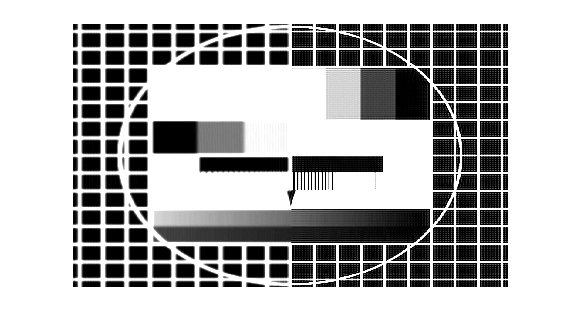
\includegraphics[width=0.7\textwidth,keepaspectratio]{../tmp/eins_c_0_1}
  \caption{komprimiertes Bild mit rechteckigem Rand im $k$-Raum, $ρ=0.1$}
  \label{fig:1c1}
\end{figure}

\section*{Aufgabe 5.1d)}

In Aufgabe d) wurde equivalent zur Verfahrensweise in c) vorgegangen.
Jedoch wurde im transformierten Raum nicht ein rechteckiger Rand abgeschnitten,
sondern ein Kreisförmiger, siehe \lref{cut_round}. Hierbei wurde darauf geachtet, dass die verbleibende
Bildinformation nach wie vor $hb\cdot ρ^2$ ist.

\lstinputlisting[firstline=1,lastline=15,firstnumber=1,label=lst:cut_round,caption={cut\_round.m}]{../code/cut_round.m}

\begin{figure}[htb]
\centering
  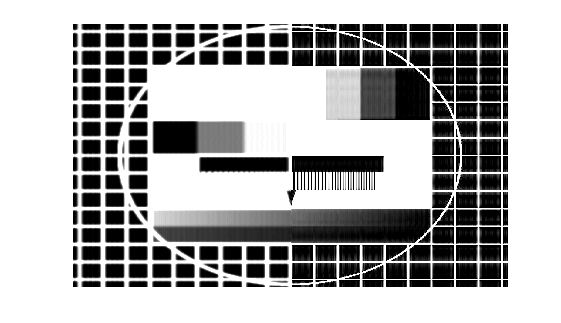
\includegraphics[width=0.7\textwidth,keepaspectratio]{../tmp/eins_c_0_5}
  \caption{komprimiertes Bild mit kreisförmigen Rand im $k$-Raum, $ρ=0.5$}
  \label{fig:1d5}
\end{figure}

\begin{figure}[htb]
\centering
  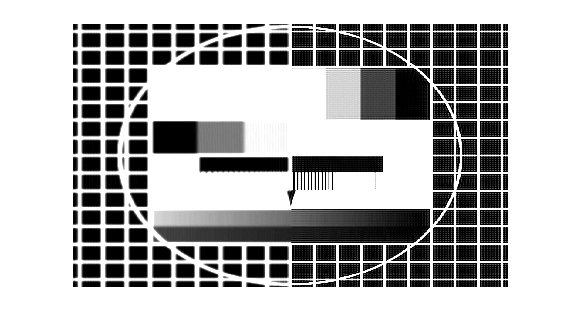
\includegraphics[width=0.7\textwidth,keepaspectratio]{../tmp/eins_c_0_1}
  \caption{komprimiertes Bild mit kreisförmigen Rand im $k$-Raum, $ρ=0.1$}
  \label{fig:1d1}
\end{figure}

Durch die Komprimierung, verändert sich das Bild. Das Ausmaß der Veränderung
hängt von der lokalen Struktur des Bildes ab. So kann man erkennen, dass
große einfarbige Flächen substrukturen aufweisen, also nicht sehr gut erhalten
bleiben. Dagegen bleiben periodische Muster, wie z.\,B. das Gitter, sehr gut
erhalten. Jedoch verschwimmen auch hier etwas Grenzen.

Farbverläufen erkennt man nach der Komprimierung deutlich die diskreten Stufen an.

Die Ergebnisse können folgendermaßen erklärt werden: Flächen entsprechen einem Plateau,
welches für eine gute Annäherung auch sehr hohe Frequenzen benötigt, welche wir jedoch
abgeschnitten haben. Daher erkennt man periodische Substrukturen.

Das Gitter selbst ist periodisch und weißt nur sehr kurze Plateaus (Peaks) auf, die auf Grund
der periodischen Natur der Fourier-Transformation im $k$-Raum auch ohne hohe Frequenzen
gut wiedergegeben werden können.

Wird eine höhere Kompression gewählt, so werden die Substrukturen deutlicher.



\section*{Aufgabe 5.1e)}